\chapter{Analisi dei requisiti}
\label{cap:analisi-requisiti}

%\intro{Breve introduzione al capitolo}\\

\section{Casi d'uso}

%Per lo studio dei casi di utilizzo del prodotto sono stati creati dei diagrammi.
%I diagrammi dei casi d'uso (in inglese \emph{Use Case Diagram}) sono diagrammi di tipo \gls{uml} dedicati alla descrizione delle funzioni o servizi offerti da un sistema, così come sono percepiti e utilizzati dagli attori che interagiscono col sistema stesso.
%Essendo il progetto finalizzato alla creazione di un tool per l'automazione di un processo, le interazioni da parte dell'utilizzatore devono essere ovviamente ridotte allo stretto necessario. Per questo motivo i diagrammi d'uso risultano semplici e in numero ridotto.

%\begin{figure}[!h] 
%    \centering 
%    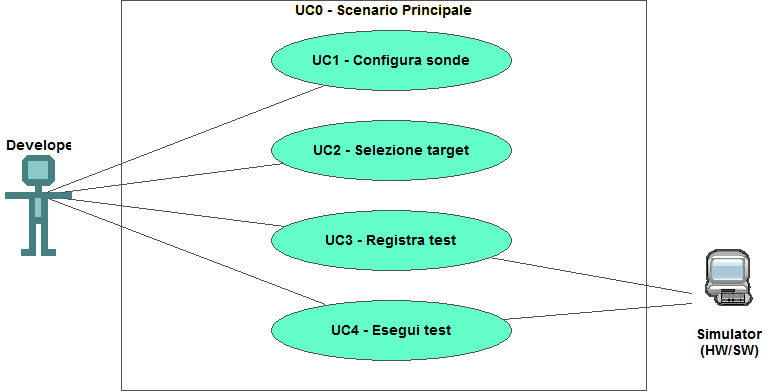
\includegraphics[width=0.9\columnwidth]{usecase/scenario-principale} 
%    \caption{Use Case - UC0: Scenario principale}
%\end{figure}
%
%\begin{usecase}{0}{Scenario principale}
%\usecaseactors{Sviluppatore applicativi}
%\usecasepre{Lo sviluppatore è entrato nel plug-in di simulazione all'interno dell'IDE}
%\usecasedesc{La finestra di simulazione mette a disposizione i comandi per configurare, registrare o eseguire un test}
%\usecasepost{Il sistema è pronto per permettere una nuova interazione}
%\label{uc:scenario-principale}
%\end{usecase}

\begin{figure}[!h] 
    \centering 
    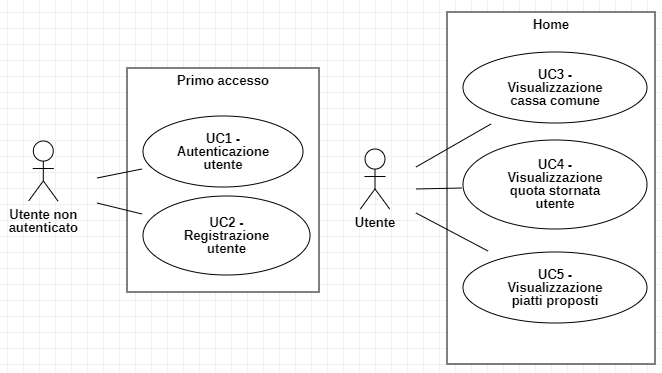
\includegraphics[width=0.9\columnwidth]{usecase/usecase-1} 
    \caption{Use Case - Primo accesso e Home}
\end{figure}

\begin{usecase}{1}{Autenticazione utente}
    \usecaseactors{Utente non autenticato}
    \usecasepre{L'utente non ha effettuato l'autenticazione}
    \usecasedesc{L'utente inserisce la propria mail e la propria password per effettuare l'accesso}
    \usecasepost{L'utente è stato autenticato}
%    \label{uc:scenario-principale}
\end{usecase}

\begin{usecase}{2}{Registrazione utente}
    \usecaseactors{Utente non autenticato}
    \usecasepre{L'utente non è registrato nel database}
    \usecasedesc{L'utente inserisce i propri dati per registrarsi nel database e effettuare l'accesso}
    \usecasepost{L'utente è stato registrato nel database}
%    \label{uc:scenario-principale}
\end{usecase}

\begin{usecase}{3}{Visualizzazione \emph{\gls{cassacomuneg}}}
    \usecaseactors{Utente}
    \usecasepre{La \emph{\gls{cassacomuneg}} non è visibile}
    \usecasedesc{L'utente entra nell'app per visualizzare la \emph{\gls{cassacomuneg}}}
    \usecasepost{L'utente visualizza la \emph{\gls{cassacomuneg}}}
%    \label{uc:scenario-principale}
\end{usecase}

\begin{usecase}{4}{Visualizzazione \emph{\gls{quotastornatag}} utente}
    \usecaseactors{Utente}
    \usecasepre{La \emph{\gls{quotastornatag}} dell'utente non è visibile}
    \usecasedesc{L'utente entra nell'app per visualizzare la \emph{\gls{quotastornatag}} dell'utente}
    \usecasepost{L'utente visualizza la \emph{\gls{quotastornatag}} dell'utente}
%    \label{uc:scenario-principale}
\end{usecase}

\begin{usecase}{5}{Visualizzazione piatti proposti}
    \usecaseactors{Utente}
    \usecasepre{La lista dei piatti proposti oggi non è visibile}
    \usecasedesc{L'utente entra nell'app per visualizzare i piatti proposti del giorno}
    \usecasepost{L'utente visualizza la lista dei piatti proposti oggi}
%    \label{uc:scenario-principale}
\end{usecase}

\newpage

\begin{figure}[!h] 
    \centering 
    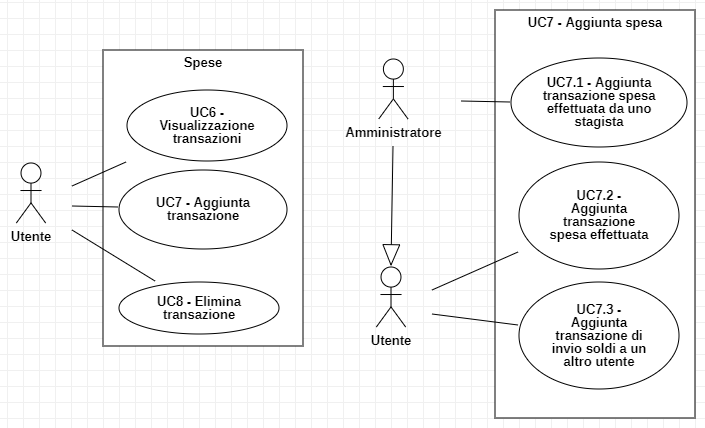
\includegraphics[width=1.0\columnwidth]{usecase/usecase-2} 
    \caption{Use Case - Spese e UC7}
\end{figure}

\begin{usecase}{6}{Visualizzazione transazioni} %serve aggiungere nel glossario la parola transazione?
    \usecaseactors{Utente}
    \usecasepre{La lista delle transazioni non è visibile}
    \usecasedesc{L'utente entra nell'app per visualizzare la lista delle transazioni}
    \usecasepost{L'utente visualizza la lista delle transazioni}
%    \label{uc:scenario-principale}
\end{usecase}

\begin{usecase}{7}{Aggiunta transazione}
    \usecaseactors{Utente}
    \usecasepre{La transazione non è presente nel database e non è visibile nella lista delle transazioni}
    \usecasedesc{L'utente inserisce i dati della transazione interessata e la salva nel database}
    \usecasepost{La transazione è presente nel database e visibile nella lista delle transazioni}
%    \label{uc:scenario-principale}
\end{usecase}

\begin{usecase}{7.1}{Aggiunta transazione spesa effettuata da uno stagista}
    \usecaseactors{Amministratore}
    \usecasepre{La spesa effettuata da un stagista non è presente nel database e non è visibile nella lista delle transazioni}
    \usecasedesc{L'amministratore inserisce i dati della spesa effettuata da un stagista e la salva nel database}
    \usecasepost{La spesa effettuata da un stagista è presente nel database e visibile nella lista delle transazioni}
%    \label{uc:scenario-principale}
\end{usecase}

\begin{usecase}{7.2}{Aggiunta transazione spesa effettuata}
    \usecaseactors{Utente}
    \usecasepre{La spesa effettuata dall'utente non è presente nel database e non è visibile nella lista delle transazioni}
    \usecasedesc{L'utente inserisce i dati della spesa effettuata e la salva nel database}
    \usecasepost{La spesa dell'utente è presente nel database e visibile nella lista delle transazioni}
%    \label{uc:scenario-principale}
\end{usecase}

\begin{usecase}{7.3}{Aggiunta transazione di invio soldi a un altro utente}
    \usecaseactors{Utente}
    \usecasepre{L'invio dei soldi ad un altro utente non è presente nel database e non è visibile nella lista delle transazioni}
    \usecasedesc{L'utente inserisce i dati dell'invio dei soldi e lo salva nel database}
    \usecasepost{L'invio dei soldi ad un altro utente è presente nel database e visibile nella lista delle transazioni}
%    \label{uc:scenario-principale}
\end{usecase}

\begin{usecase}{8}{Elimina transazione}
    \usecaseactors{Utente}
    \usecasepre{La transazione è presente nel database e visibile nella lista delle transazioni}
    \usecasedesc{L'utente elimina la transazione interessata dall'app e viene eliminata dal database}
    \usecasepost{La transazione non è presente nel database e non è visibile nella lista delle transazioni}
%    \label{uc:scenario-principale}
\end{usecase}

\newpage

\begin{figure}[!h] 
    \centering 
    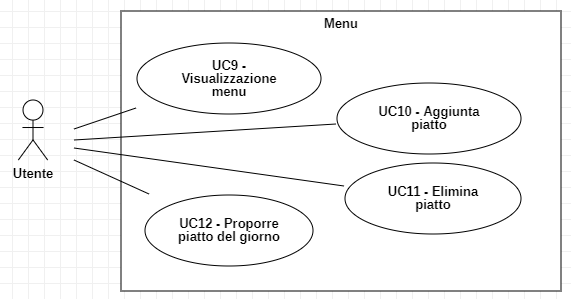
\includegraphics[width=0.8\columnwidth]{usecase/usecase-3} 
    \caption{Use Case - Menu}
\end{figure}

\begin{usecase}{9}{Visualizzazione menu} %serve aggiungere nel glossario la parola transazione?
    \usecaseactors{Utente}
    \usecasepre{Il menu non è visibile}
    \usecasedesc{L'utente entra nell'app per visualizzare il menu}
    \usecasepost{L'utente visualizza la lista dei piatti presenti nel menu}
%    \label{uc:scenario-principale}
\end{usecase}

\begin{usecase}{10}{Aggiunta piatto}
    \usecaseactors{Utente}
    \usecasepre{Il piatto non è presente nel database e non è visibile nel menu}
    \usecasedesc{L'utente inserisce i dati del piatto e lo salva nel database}
    \usecasepost{Il piatto è presente nel database e visibile nel menu}
%    \label{uc:scenario-principale}
\end{usecase}

\begin{usecase}{11}{Elimina piatto}
    \usecaseactors{Utente}
    \usecasepre{Il piatto è presente nel database e visibile dal menu}
    \usecasedesc{L'utente elimina il piatto interessata dall'app e viene eliminato dal database}
    \usecasepost{Il piatto non è presente nel database e non è visibile nel menu}
%    \label{uc:scenario-principale}
\end{usecase}

\begin{usecase}{12}{Proporre piatto del giorno}
    \usecaseactors{Utente}
    \usecasepre{Il piatto non è indicato come piatto proposto del giorno}
    \usecasedesc{L'utente propone il piatto interessato come piatto del giorno}
    \usecasepost{Il piatto è indicato come piatto proposto del giorno}
%    \label{uc:scenario-principale}
\end{usecase}

\newpage

\begin{figure}[!h] 
    \centering 
    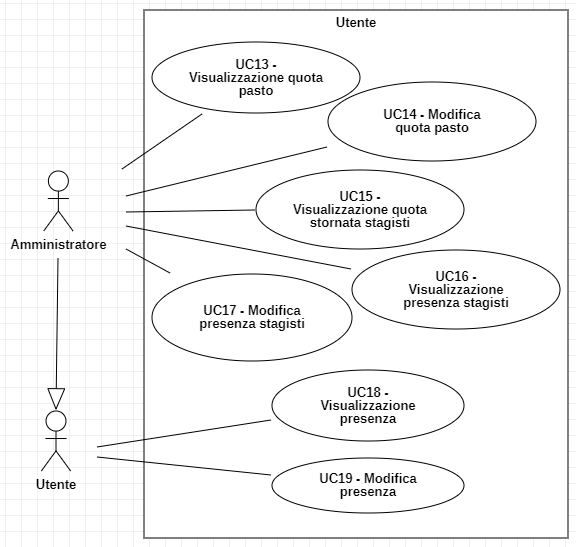
\includegraphics[width=0.9\columnwidth]{usecase/usecase-4} 
    \caption{Use Case - Utente}
\end{figure}

\begin{usecase}{13}{Visualizzazione quota pasto} %aggiungere nel glossario quota pasto
    \usecaseactors{Amministratore}
    \usecasepre{La quota pasto non è visibile}
    \usecasedesc{L'amministratore entra nell'app per visualizzare la quota pasto}
    \usecasepost{L'amministratore visualizza la quota pasto}
%    \label{uc:scenario-principale}
\end{usecase}

\begin{usecase}{14}{Modifica quota pasto} %aggiungere nel glossario quota pasto
    \usecaseactors{Amministratore}
    \usecasepre{La quota pasto è salvata nel database con il vecchio valore}
    \usecasedesc{L'amministratore modifica la quota pasto con il nuovo valore}
    \usecasepost{La quota passto è salvata nel database con il nuovo valore}
%    \label{uc:scenario-principale}
\end{usecase}

\begin{usecase}{15}{Visualizzazione \emph{\gls{quotastornatag}} stagisti}
    \usecaseactors{Amministratore}
    \usecasepre{La \emph{\gls{quotastornatag}} stagisti non è visibile}
    \usecasedesc{L'amministratore entra nell'app per visualizzare la \emph{\gls{quotastornatag}} stagisti}
    \usecasepost{L'amministratore visualizza la \emph{\gls{quotastornatag}} stagisti}
%    \label{uc:scenario-principale}
\end{usecase}

\begin{usecase}{16}{Visualizzazione presenza stagisti}
    \usecaseactors{Amministratore}
    \usecasepre{La lista delle presenze dei stagisti non è visibile}
    \usecasedesc{L'amministratore entra nell'app per visualizzare la lista delle presenze dei stagisti}
    \usecasepost{L'amministratore visualizza la lista delle presenze dei stagisti}
%    \label{uc:scenario-principale}
\end{usecase}

\begin{usecase}{17}{Modifica presenza stagisti}
    \usecaseactors{Amministratore}
    \usecasepre{La lista delle presenze degli stagisti è salvato nel database con i vecchi valori}
    \usecasedesc{L'amministratore modifica la lista delle presenze degli stagisti con i nuovi valori}
    \usecasepost{La lista delle presenze degli stagisti è salvato nel database con i nuovi valori}
%    \label{uc:scenario-principale}
\end{usecase}

\begin{usecase}{18}{Visualizzazione presenza}
    \usecaseactors{Utente}
    \usecasepre{La lista delle presenze dell'utente non è visibile}
    \usecasedesc{L'utente entra nell'app per visualizzare la lista delle proprie presenze}
    \usecasepost{L'utente visualizza la lista delle proprie presenze}
%    \label{uc:scenario-principale}
\end{usecase}

\begin{usecase}{19}{Modifica presenza}
    \usecaseactors{Amministratore}
    \usecasepre{La lista delle presenze dell'utente è salvato nel database con i vecchi valori}
    \usecasedesc{L'utente modifica la lista delle proprie presenze con i nuovi valori}
    \usecasepost{La lista delle presenze dell'utente è salvato nel database con i nuovi valori}
%    \label{uc:scenario-principale}
\end{usecase}

\newpage

\begin{figure}[!h] 
    \centering 
    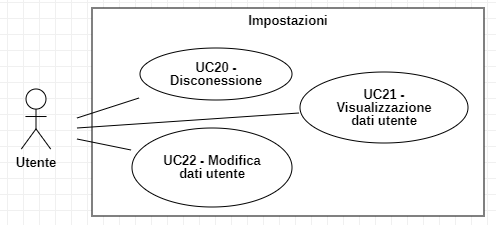
\includegraphics[width=0.7\columnwidth]{usecase/usecase-5} 
    \caption{Use Case - Impostazioni}
\end{figure}

\begin{figure}[!h] 
    \centering 
    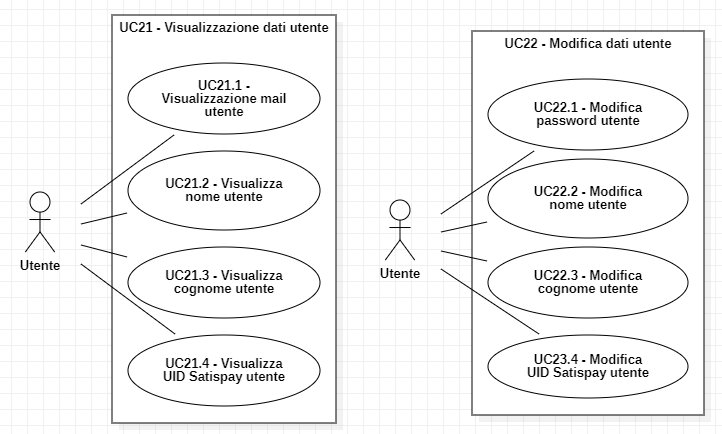
\includegraphics[width=1.1\columnwidth]{usecase/usecase-6} 
    \caption{Use Case - UC21 e UC22}
\end{figure}

\begin{usecase}{20}{Disconnessione}
    \usecaseactors{Utente}
    \usecasepre{L'utente è autenticato nell'app}
    \usecasedesc{L'utente disconnette l'accesso effettuato}
    \usecasepost{L'utente non è autenticato}
%    \label{uc:scenario-principale}
\end{usecase}

\begin{usecase}{21}{Visualizzazione dati utente}
    \usecaseactors{Utente}
    \usecasepre{I dati dell'utente non sono visibili}
    \usecasedesc{L'utente entra nell'app per visualizzare i propri dati}
    \usecasepost{L'utente visualizza i propri dati}
%    \label{uc:scenario-principale}
\end{usecase}

\begin{usecase}{21.1}{Visualizzazione mail utente}
    \usecaseactors{Utente}
    \usecasepre{La mail dell'utente non è visibile}
    \usecasedesc{L'utente entra nell'app per visualizzare la propria mail}
    \usecasepost{L'utente visualizza la propria mail}
%    \label{uc:scenario-principale}
\end{usecase}

\begin{usecase}{21.2}{Visualizzazione nome utente}
    \usecaseactors{Utente}
    \usecasepre{Il nome dell'utente non è visibile}
    \usecasedesc{L'utente entra nell'app per visualizzare il proprio nome}
    \usecasepost{L'utente visualizza il proprio nome}
%    \label{uc:scenario-principale}
\end{usecase}

\begin{usecase}{21.3}{Visualizzazione cognome utente}
    \usecaseactors{Utente}
    \usecasepre{Il cognome dell'utente non è visibile}
    \usecasedesc{L'utente entra nell'app per visualizzare il proprio cognome}
    \usecasepost{L'utente visualizza il proprio cognome}
%    \label{uc:scenario-principale}
\end{usecase}

\begin{usecase}{21.4}{Visualizzazione UID Satispay utente}
    \usecaseactors{Utente}
    \usecasepre{L'UID Satispay dell'utente non è visibile}
    \usecasedesc{L'utente entra nell'app per visualizzare il proprio UID Satispay}
    \usecasepost{L'utente visualizza il proprio UID Satispay}
%    \label{uc:scenario-principale}
\end{usecase}

\begin{usecase}{22}{Modifica dati utente}
    \usecaseactors{Utente}
    \usecasepre{I dati dell'utente sono salvati nel database con i vecchi valori}
    \usecasedesc{L'utente modifica i propri dati con i nuovi valori}
    \usecasepost{I dati dell'utente sono salvati nel database con i nuovi valori}
%    \label{uc:scenario-principale}
\end{usecase}

\begin{usecase}{22.1}{Modifica password utente}
    \usecaseactors{Utente}
    \usecasepre{La password dell'utente è salvato nel database con il vecchio valore}
    \usecasedesc{L'utente modifica la propria password con il nuovo valore}
    \usecasepost{La password dell'utente è salvato nel database con il nuovo valore}
%    \label{uc:scenario-principale}
\end{usecase}

\begin{usecase}{22.2}{Modifica nome utente}
    \usecaseactors{Utente}
    \usecasepre{Il nome dell'utente è salvato nel database con il vecchio valore}
    \usecasedesc{L'utente modifica il proprio nome con il nuovo valore}
    \usecasepost{Il nome dell'utente è salvato nel database con il nuovo valore}
%    \label{uc:scenario-principale}
\end{usecase}

\begin{usecase}{22.3}{Modifica cognome utente}
    \usecaseactors{Utente}
    \usecasepre{Il cognome dell'utente è salvato nel database con il vecchio valore}
    \usecasedesc{L'utente modifica il proprio cognome con il nuovo valore}
    \usecasepost{Il cognome dell'utente è salvato nel database con il nuovo valore}
%    \label{uc:scenario-principale}
\end{usecase}

\begin{usecase}{22.4}{Modifica UID Satispay utente}
    \usecaseactors{Utente}
    \usecasepre{L'UID di Satispay dell'utente è salvato nel database con il vecchio valore}
    \usecasedesc{L'utente modifica il proprio UID Satispay con il nuovo valore}
    \usecasepost{L'UID Satispay dell'utente è salvato nel database con il nuovo valore}
%    \label{uc:scenario-principale}
\end{usecase}

\newpage

\section{Tracciamento dei requisiti}

%Da un'attenta analisi dei requisiti e degli use case effettuata sul progetto è stata stilata la tabella che traccia i requisiti in rapporto agli use case.\\
%Sono stati individuati diversi tipi di requisiti e si è quindi fatto utilizzo di un codice identificativo per distinguerli.\\
%Il codice dei requisiti è così strutturato R(O/D/F) dove:
%\begin{enumerate}
%%	\item[R =] requisito
%%    \item[F =] funzionale
%%    \item[Q =] qualitativo
%%    \item[V =] di vincolo
%    \item[O =] obbligatorio (necessario)
%    \item[D =] desiderabile
%    \item[F =] facoltativo
%%    \item[Z =] opzionale
%\end{enumerate}
%Nelle tabelle \ref{tab:requisiti-obbligatori}, \ref{tab:requisiti-desiderabili} e \ref{tab:requisiti-facoltativi} sono riassunti i requisiti e il loro tracciamento con gli use case delineati in fase di analisi.
%
%\newpage
%
%\begin{table}%
%\caption{Tabella del tracciamento dei requisti obbligatori}
%\label{tab:requisiti-obbligatori}
%\begin{tabularx}{\textwidth}{lXl}
%\hline\hline
%\textbf{Requisito} & \textbf{Descrizione} & \textbf{Use Case}\\
%\hline
%RO-1     & L'interfaccia permette di configurare il tipo di sonde del test & UC1 \\
%\hline
%\end{tabularx}
%\end{table}%
%
%\begin{table}%
%\caption{Tabella del tracciamento dei requisiti desiderabili}
%\label{tab:requisiti-desiderabili}
%\begin{tabularx}{\textwidth}{lXl}
%\hline\hline
%\textbf{Requisito} & \textbf{Descrizione} & \textbf{Use Case}\\
%\hline
%RD-1    & Le prestazioni del simulatore hardware deve garantire la giusta esecuzione dei test e non la generazione di falsi negativi & - \\
%\hline
%\end{tabularx}
%\end{table}%
%
%\begin{table}%
%\caption{Tabella del tracciamento dei requisiti facoltativi}
%\label{tab:requisiti-facoltativi}
%\begin{tabularx}{\textwidth}{lXl}
%\hline\hline
%\textbf{Requisito} & \textbf{Descrizione} & \textbf{Use Case}\\
%\hline
%RF-1    & La libreria per l'esecuzione dei test automatici deve essere riutilizzabile & - \\
%\hline
%\end{tabularx}
%\end{table}%
